\documentclass[DIN, pagenumber=false, fontsize=11pt, parskip=half]{scrartcl}

\usepackage{amsmath}
\usepackage{amsfonts}
\usepackage{amssymb}
\usepackage{enumitem}
\usepackage[utf8]{inputenc} 
\usepackage[ngerman]{babel} 
\usepackage[T1]{fontenc} 
\usepackage{pgfplots}
\usepackage{xcolor}
\usepackage{listings}
\usepackage{float}
\usepackage{graphicx}
\usepackage{svg}
\usepackage{booktabs}
\usepackage{gensymb}
\usepackage{dcolumn}


\definecolor{mygreen}{RGB}{28,172,0} % color values Red, Green, Blue
\definecolor{mylilas}{RGB}{170,55,241}

\newcommand{\norm}[1]{\left\lVert#1\right\rVert}

\lstset{language=Matlab,%
    %basicstyle=\color{red},
    breaklines=true,%
    morekeywords={matlab2tikz},
    keywordstyle=\color{blue},%
    morekeywords=[2]{1}, keywordstyle=[2]{\color{black}},
    identifierstyle=\color{black},%
    stringstyle=\color{mylilas},
    commentstyle=\color{mygreen},%
    showstringspaces=false,%without this there will be a symbol in the places where there is a space
    numbers=left,%
    numberstyle={\tiny \color{black}},% size of the numbers
    numbersep=9pt, % this defines how far the numbers are from the text
    emph=[1]{for,end,break},emphstyle=[1]\color{red}, %some words to emphasise
    %emph=[2]{word1,word2}, emphstyle=[2]{style},    
}

\DeclareUnicodeCharacter{00B0}{\degree}


\title{Computer Vision I}
\author{Tim Luchterhand, Paul Nykiel (Group 17)}

\begin{document}
    \maketitle
    \section{Gaussian Pyramids}
    \lstinputlisting{sh05ex01.m}
    \begin{figure}[H]
        \centering
        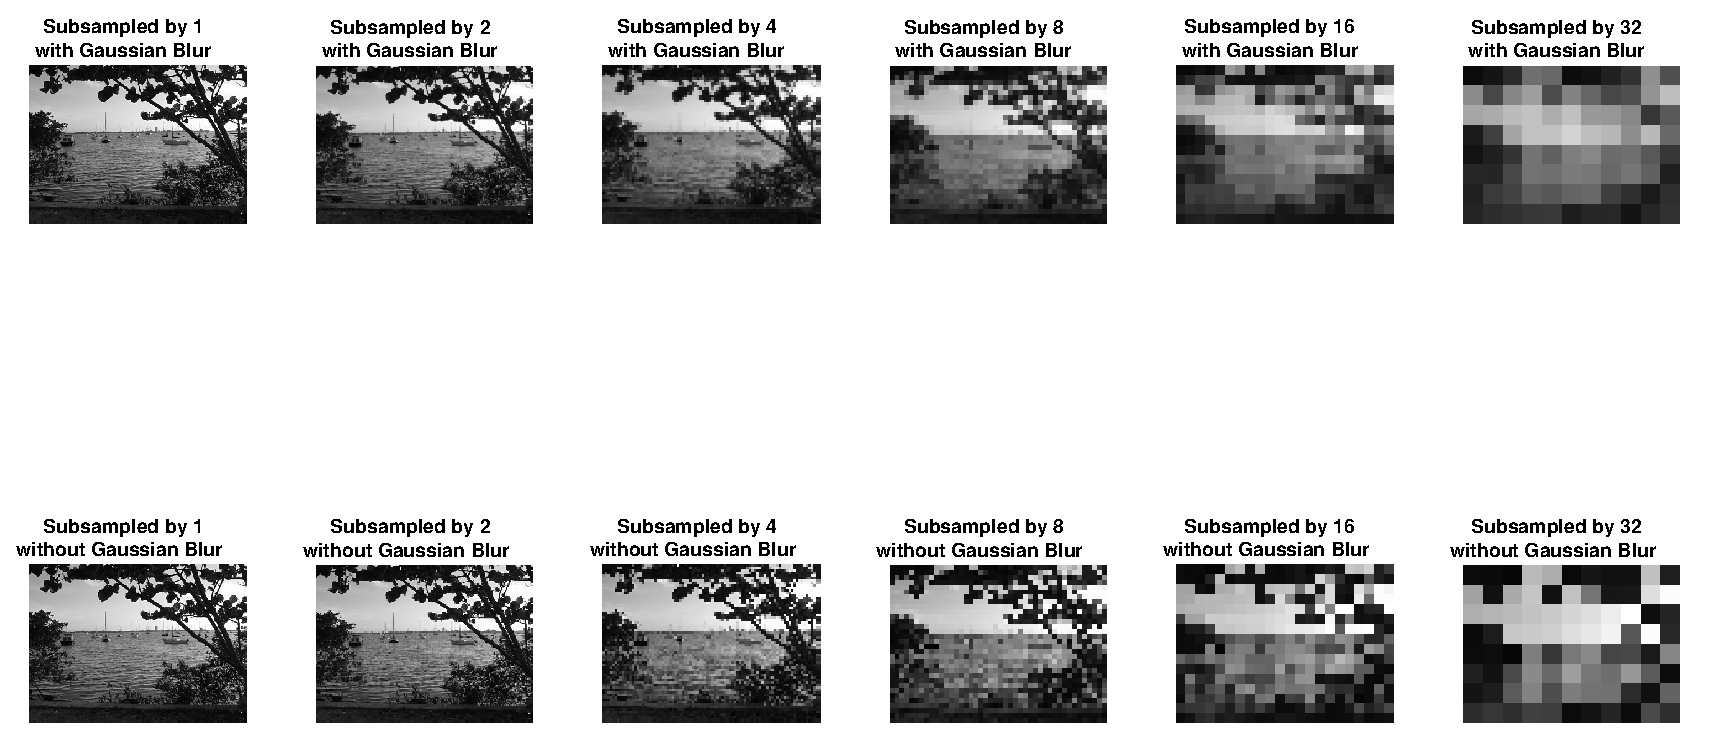
\includegraphics[width=\textwidth]{sh05ex01.eps}
        \caption{Output of the matlab script}
    \end{figure}

    \section{Laplacian Pyramids}
    \subsection{}
    \lstinputlisting[firstline=1, firstnumber=1, lastline=36]{sh05ex02.m}
    \begin{figure}[H]
        \centering
        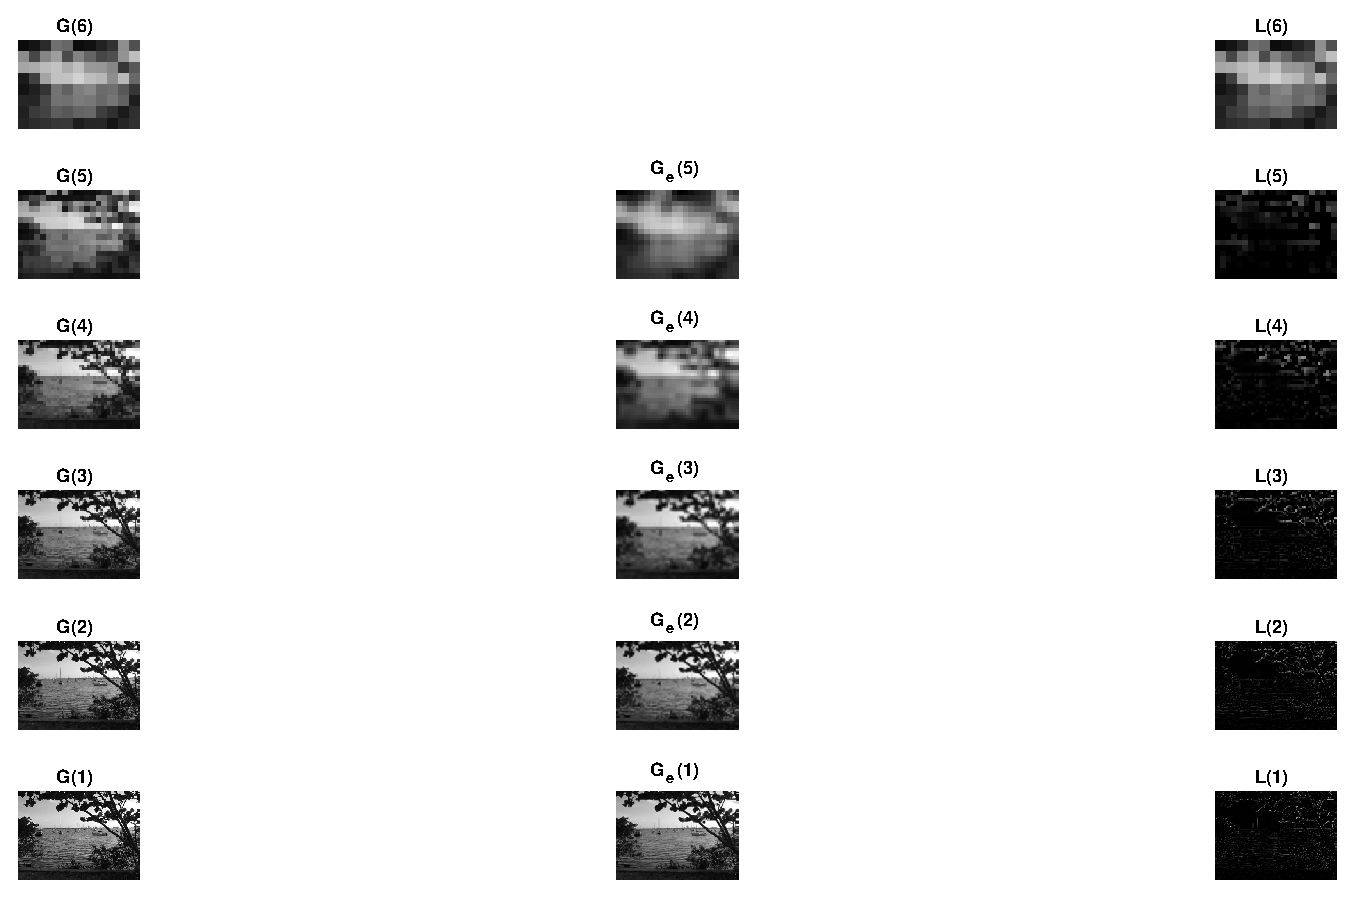
\includegraphics[width=\textwidth]{sh05ex02_1.eps}
        \caption{Output of the matlab script}
    \end{figure}

    \subsection{}
    \lstinputlisting[firstline=38, firstnumber=38, lastline=64]{sh05ex02.m}
    \begin{figure}[H]
        \centering
        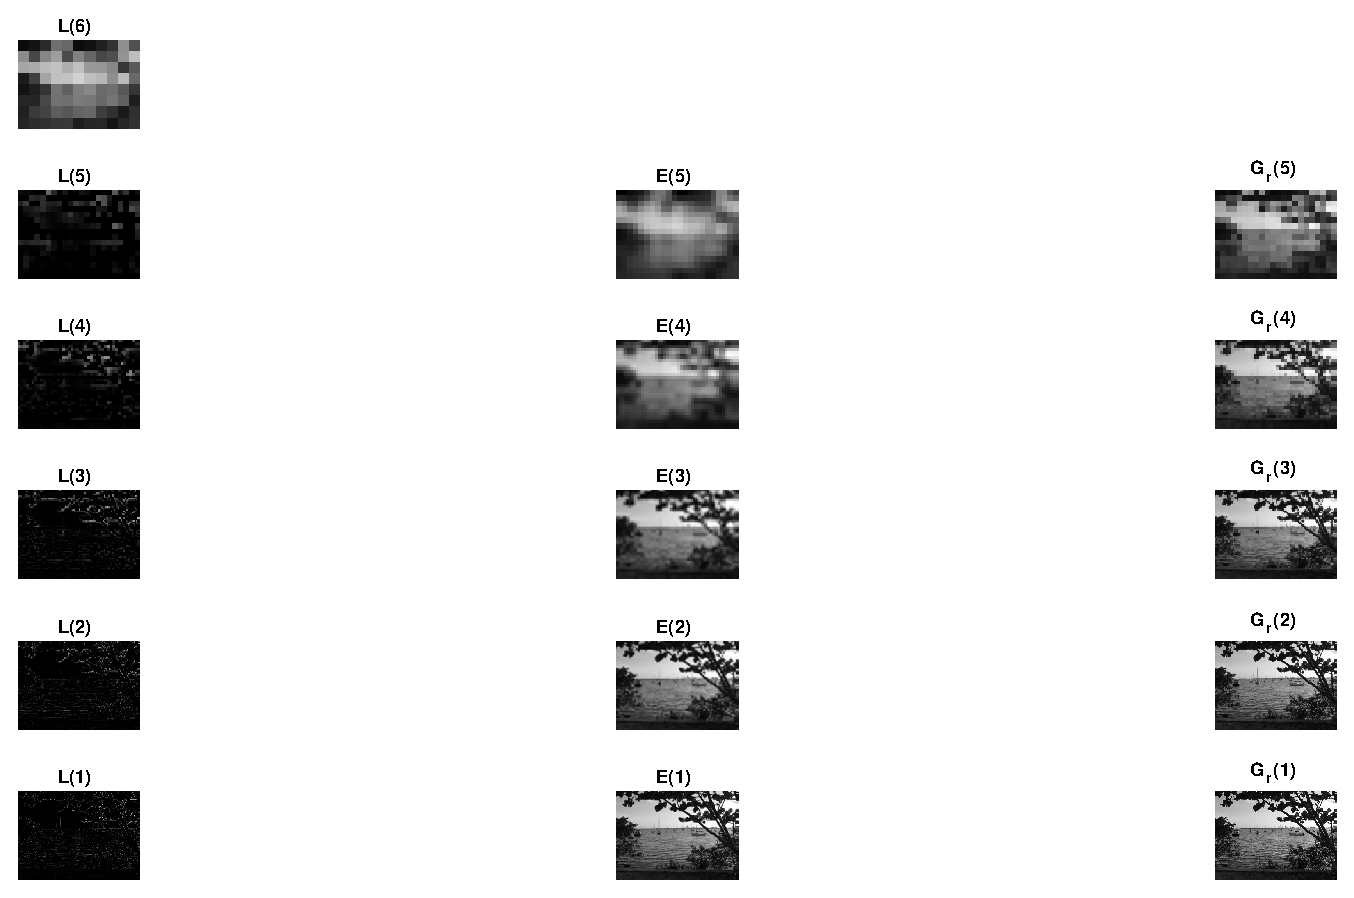
\includegraphics[width=\textwidth]{sh05ex02_2.eps}
        \caption{Output of the matlab script}
    \end{figure}

    \subsection{}
    \lstinputlisting[firstline=66, firstnumber=66, lastline=107]{sh05ex02.m}
    \begin{figure}[H]
        \centering
        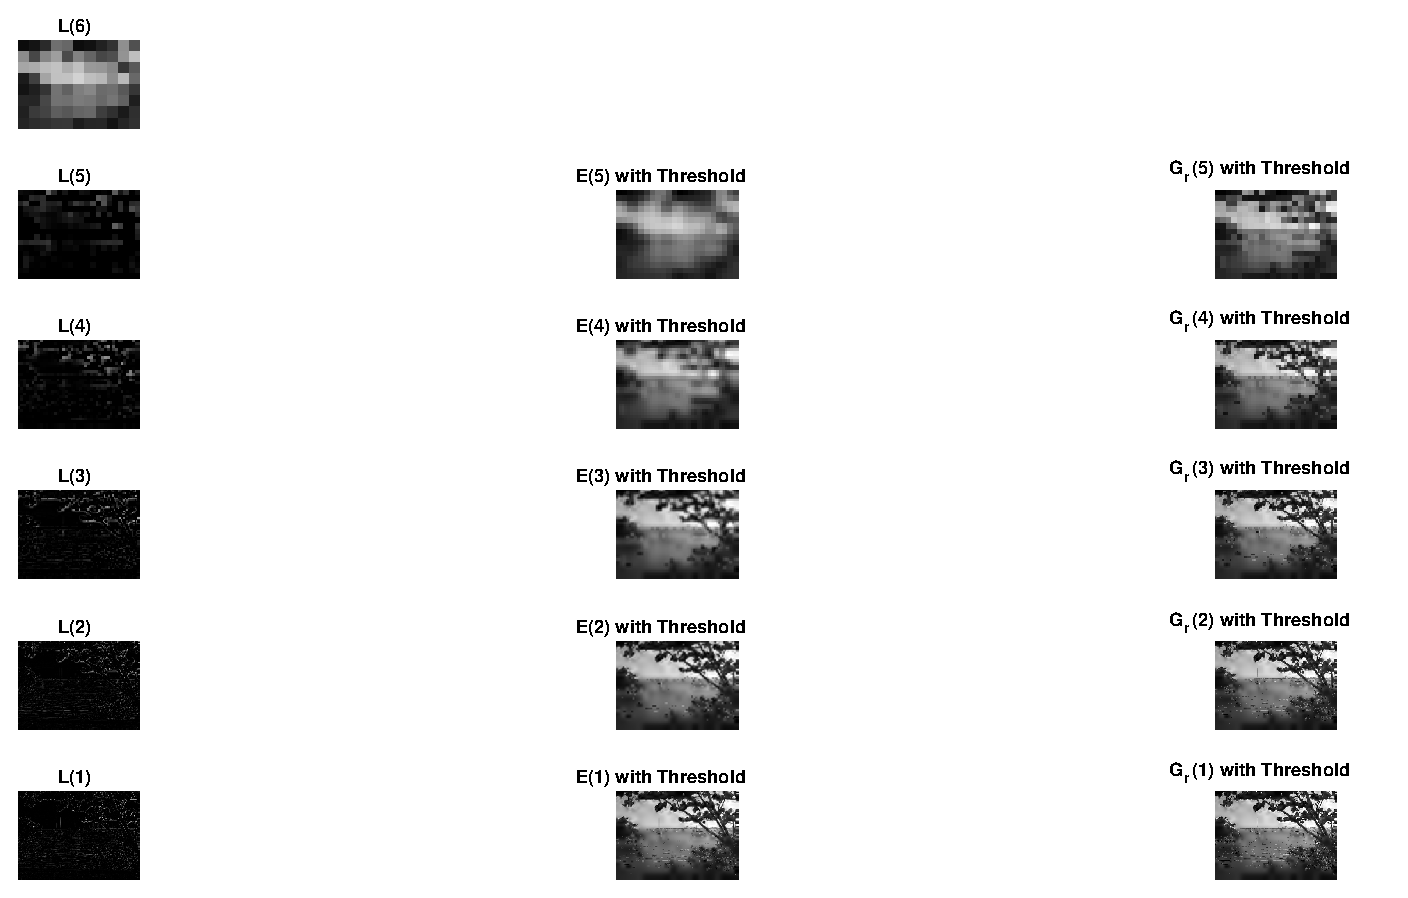
\includegraphics[width=\textwidth]{sh05ex02_3_1.eps}
        \caption{Output of the matlab script}
    \end{figure}
    \begin{figure}[H]
        \centering
        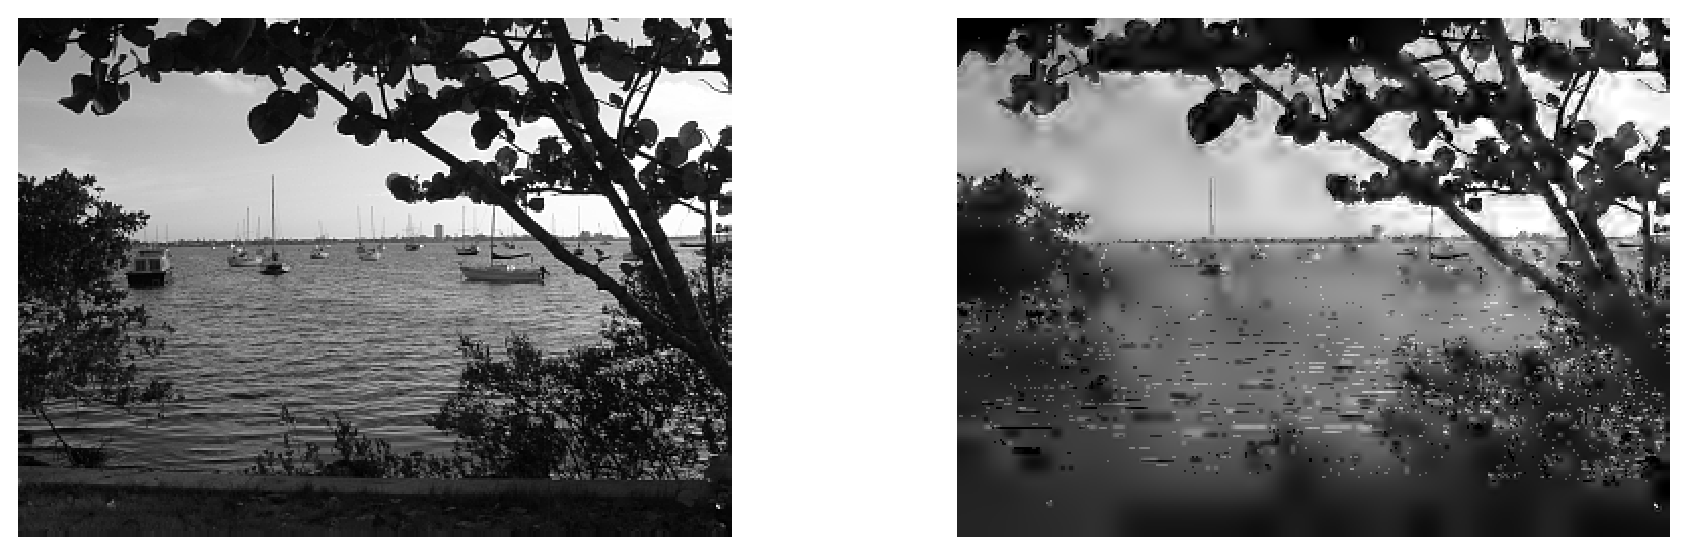
\includegraphics[width=\textwidth]{sh05ex02_3_2.eps}
        \caption{Difference between the reconstructed and the original image}
    \end{figure}

    \subsection{}
    \lstinputlisting[firstline=109, firstnumber=109]{sh05ex02.m}
    \begin{figure}[H]
        \centering
        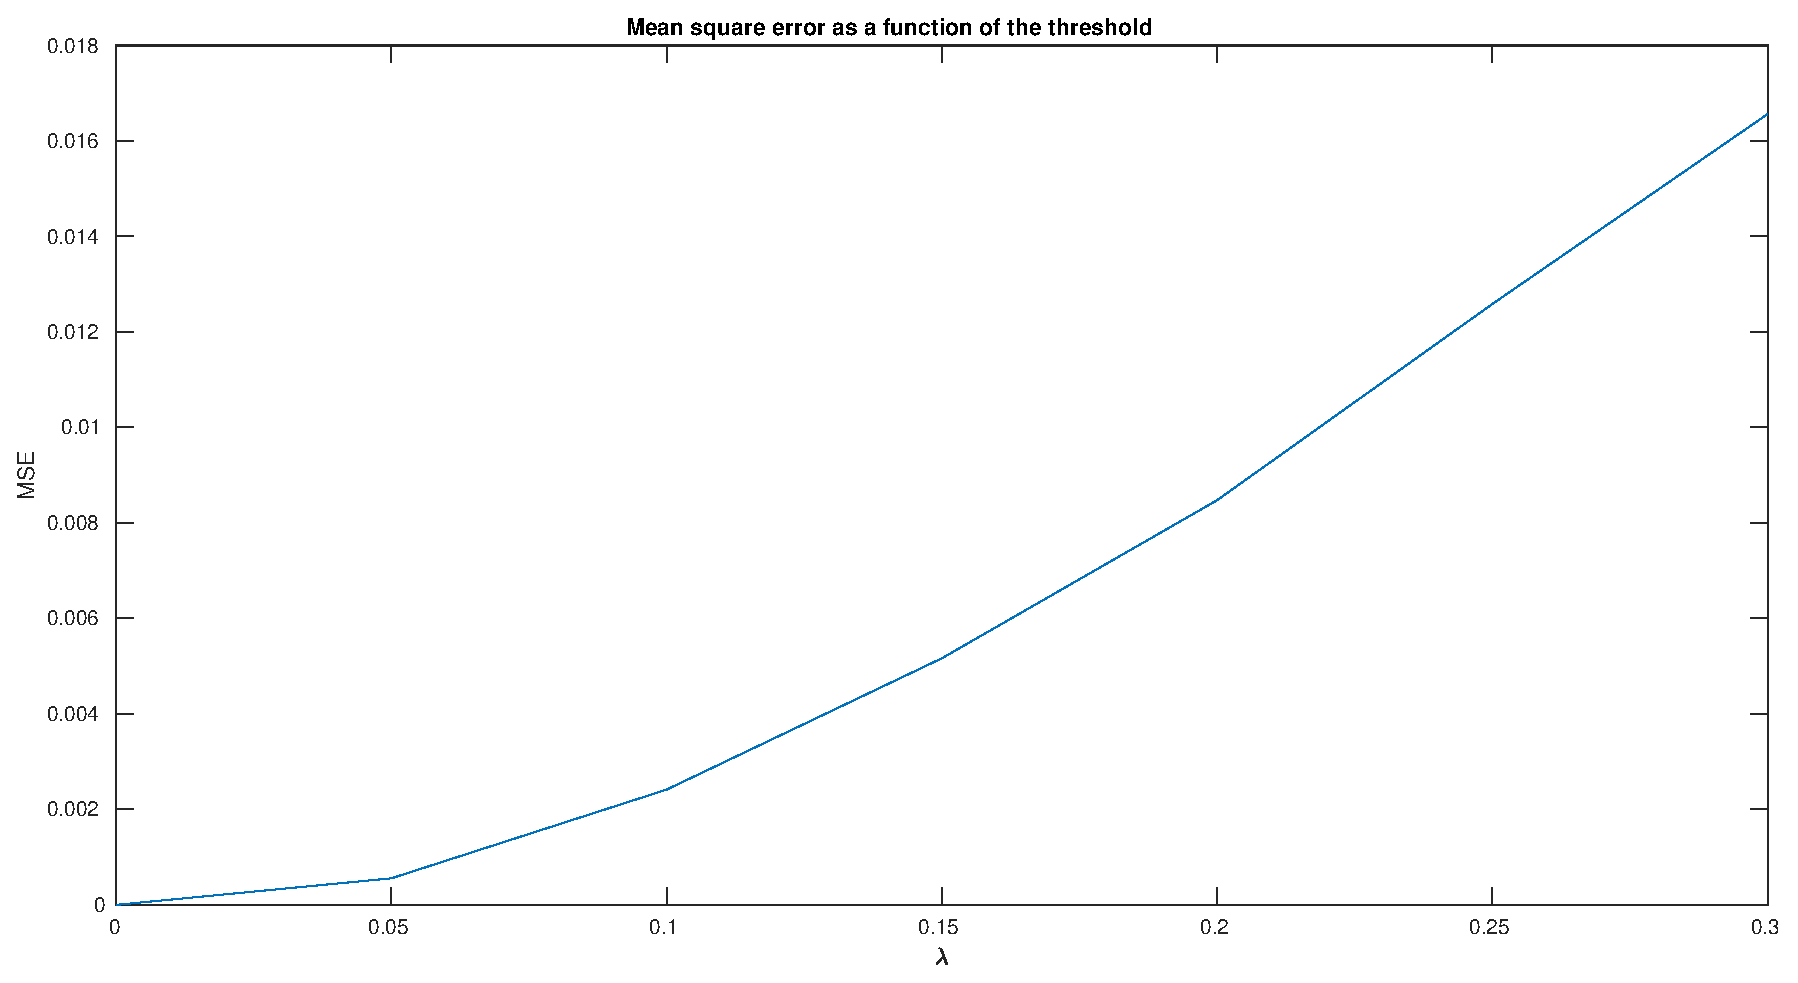
\includegraphics[width=\textwidth]{sh05ex02_4.eps}
        \caption{Output of the matlab script}
    \end{figure}

    \section{Gabor Wavelets}
    \lstinputlisting{sh05ex03.m}
    \begin{figure}[H]
        \centering
        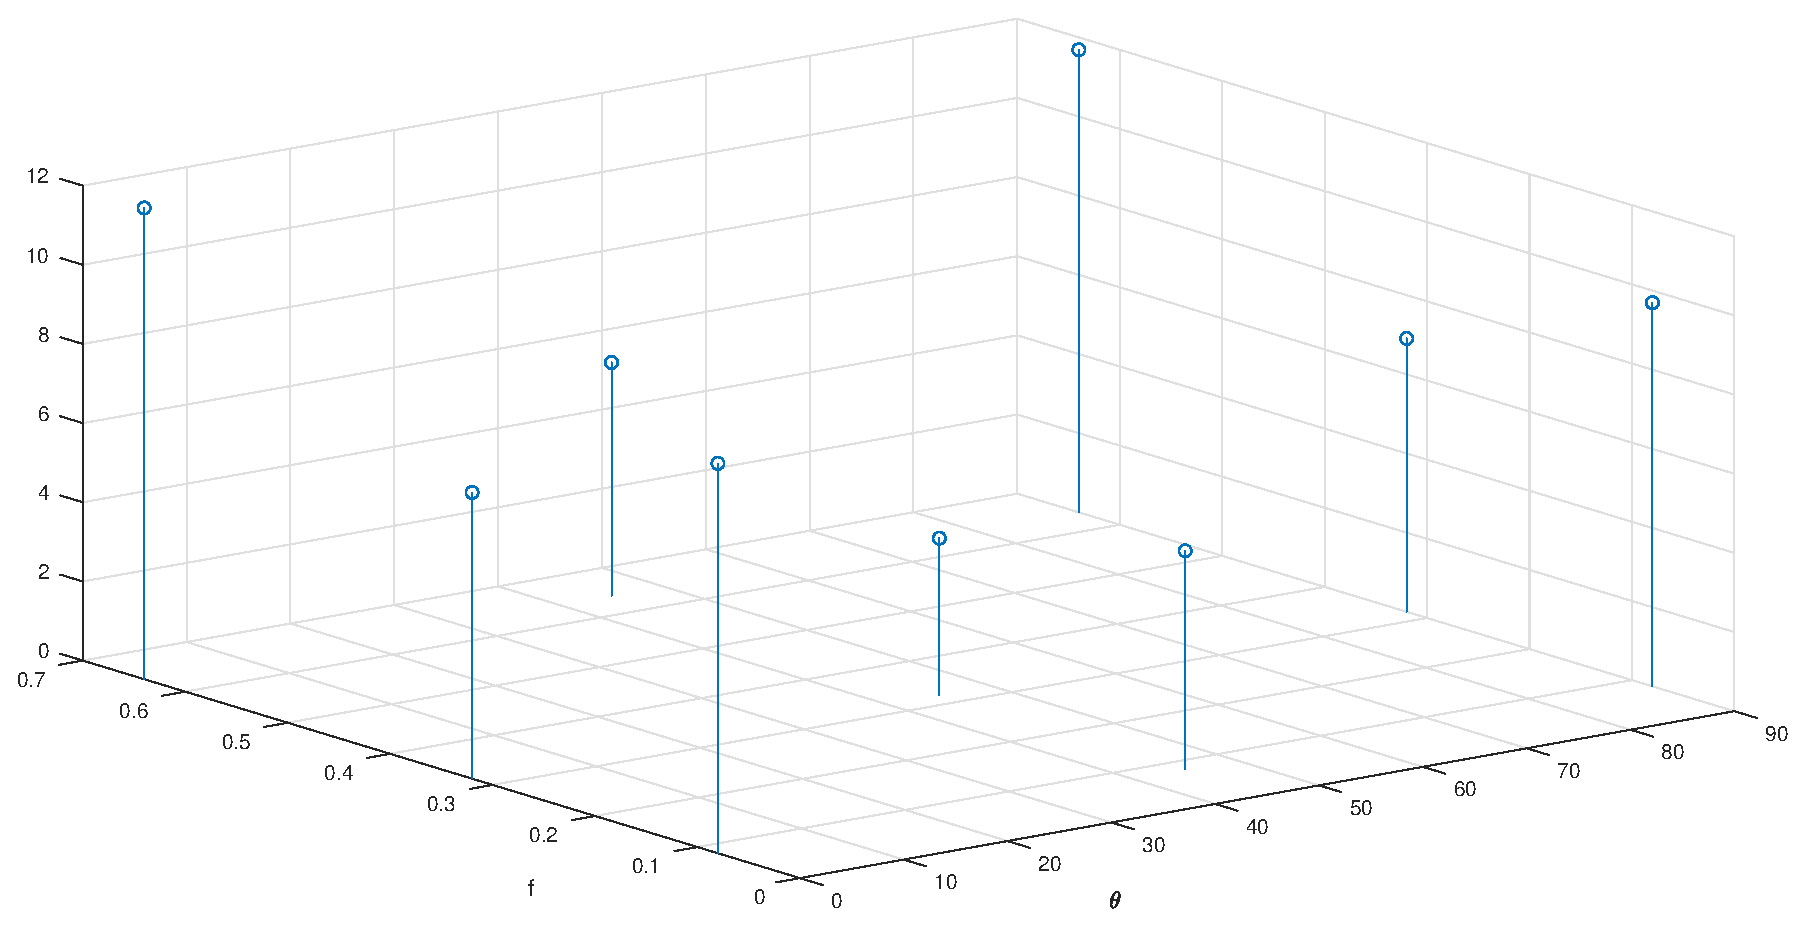
\includegraphics[width=\textwidth]{sh05ex03.eps}
        \caption{Output of the matlab script}
    \end{figure}
    For the orientation $\theta = 45 \degree$ all the frequency energys are lower compared to the other orientations since there are no significant image structures
    like edges.

    In the other directions ($\theta = 0 \degree$ and $\theta = 90\degree$) there are peaks at high frequencys due to prominent edges, as well as peaks at low
    frequencys as a result of partitally homogeneous regions.
\end{document}
